% =====================================================================================
%  Self-Healing Agents: An Evidence-Gated Rule-Learning Harness for Reliable LLM Agents
%  Anonymized double-blind AAAI 2027 submission draft.
%  Uses the official AAAI 2027 author-kit style (aaai2027.sty + aaai2027.bst).
%  Build with PDFLaTeX (the aaai2027 style requires it -- it will NOT compile under
%  XeLaTeX / LuaLaTeX / tectonic; Overleaf's default pdfLaTeX works):
%      pdflatex main && bibtex main && pdflatex main && pdflatex main
%  Undefined-CITATION warnings from the clearly-marked placeholder bib keys are expected.
% =====================================================================================
\documentclass[letterpaper]{article} % DO NOT CHANGE THIS
\usepackage[submission]{aaai2027}  % DO NOT CHANGE THIS
% Fonts (newtxtext / helvet / courier) are loaded automatically by aaai2027.sty.
% DO NOT add times/helvet/courier or any other font package.
\usepackage[hyphens]{url}  % DO NOT CHANGE THIS
\usepackage{graphicx} % DO NOT CHANGE THIS
\urlstyle{rm} % DO NOT CHANGE THIS
\def\UrlFont{\rm}  % DO NOT CHANGE THIS
\usepackage{natbib}  % DO NOT CHANGE THIS AND DO NOT ADD ANY OPTIONS TO IT
\usepackage{caption} % DO NOT CHANGE THIS AND DO NOT ADD ANY OPTIONS TO IT
\frenchspacing  % DO NOT CHANGE THIS
\setcounter{secnumdepth}{2} % number sections + subsections (we cross-reference them via \S\ref)

% Algorithms (AAAI-recommended packages).
\usepackage{algorithm}
\usepackage{algorithmic}

% Better-looking tables.
\usepackage{booktabs}

% Math and figure drawing. None of these are on the AAAI disallowed list
% (pgfplots IS disallowed and is not used; tikz draws the two schematic figures).
\usepackage{amsmath,amssymb}
\usepackage{tikz}
\usetikzlibrary{arrows.meta,positioning,fit,backgrounds,calc}

% Keep \pdfinfo as-is (the [submission] option turns it into a no-op).
\pdfinfo{
/TemplateVersion (2027.1)
}

% --- notation macros (keep symbols consistent everywhere, incl. results) ---
\newcommand{\ind}{\mathbf{1}}                     % indicator
\newcommand{\Rset}{\mathcal{R}}                   % active/candidate rule set
\newcommand{\evalfn}{\mathcal{E}}                 % session-level evaluation service
\newcommand{\mvec}{\mathbf{m}}                    % metric vector
\newcommand{\Heal}{\mathcal{H}}                   % self-heal operator
\newcommand{\Breach}{\mathfrak{B}}                % observed breaches
\newcommand{\dpromote}{\delta_{\mathrm{prom}}}
\newcommand{\dregress}{\delta_{\mathrm{reg}}}
\newcommand{\passk}{\mathrm{pass}^{k}}
\newcommand{\passone}{\mathrm{pass@}1}
\newcommand{\TBD}{--}                             % placeholder cell (numbers forthcoming)
\newcommand{\topk}{\textsc{top-}k}

% Title in Title Case (AAAI requirement). Author auto-anonymized by the [submission] option.
\title{Self-Healing Agents: An Evidence-Gated Rule-Learning Harness for Reliable LLM Agents}
\author{Anonymous Submission}
\affiliations{} % leave empty for anonymous review (AAAI guideline)

\begin{document}
\maketitle

% =====================================================================================
\begin{abstract}
Large language model (LLM) agents that are \emph{capable} on a task are not necessarily
\emph{reliable} on it: the same agent, run repeatedly, frequently succeeds on some trials and
fails on others, and quality tends to drift over long horizons. Peak-performance metrics such
as $\passone$ hide this variance, whereas the stricter reliability metric $\passk$---the
fraction of tasks solved on \emph{all} $k$ independent trials---exposes it. We present a
\emph{self-healing agent harness} (hereafter \emph{the Harness}): a runtime envelope that wraps
an arbitrary LLM agent loop and, with no human in the loop, (i) \emph{detects} its own quality
degradations from a session-level agent-evaluation service, (ii) posts structured diagnostic
notices to a workspace that the agent \emph{pulls} on its own initiative---nothing is injected
into the conversation, (iii) lets the agent author corrective operating \emph{rules}, and (iv)
admits each rule only after it passes an empirical \emph{evidence gate}: a replay of the
captured failure or a forward trial over subsequent live sessions, with a regression guard
against forgetting past wins. We formalize the loop as an evidence-gated operator on the
agent's policy-inducing context and cast rule validation as paired empirical improvement
testing with a multi-metric non-regression constraint. We evaluate the Harness with an A/B
protocol (identical agent, baseline vs.\ Harness) across three agent benchmarks spanning tool
use, digital work, and terminal tasks, reporting $\passone$ and $\passk$ with paired
significance tests. \textbf{Findings are forthcoming:} the study's runs are in progress; the
Harness is designed to raise $\passk$ (reliability) more than $\passone$ (peak
capability)---the headline effect is a placeholder [TODO] pending completion of the runs.
\end{abstract}

% =====================================================================================
\section{Introduction}
\label{sec:intro}

Progress on LLM agents is usually reported as \emph{capability}: can the agent, at its best,
solve the task? But deployment demands \emph{reliability}: does it solve the task \emph{every}
time it is asked? These are different properties, and the gap between them is large. Because
modern agents are stochastic---and, increasingly, because frontier models do not expose a
temperature control, so sampling variation cannot even be turned off---repeated runs of the
same agent on the same task yield different outcomes. A metric like $\passone$ (did the first
trial pass?) rewards a lucky draw; the stricter $\passk$ (did \emph{all} $k$ independent trials
pass?) is a direct measure of reliability and is typically far lower. Closing this
\emph{reliability gap} is the problem we attack.

A natural idea is to let the agent correct itself. A rich line of work does exactly this
\emph{within an episode}: the agent reflects on a failed attempt and retries
\citep{placeholder-reflexion,placeholder-selfrefine,placeholder-critic}. Such open-loop
self-correction has two limitations that matter for reliability. First, it is
\emph{unvalidated}: a reflection that \emph{sounds} corrective is trusted immediately, even
though a plausible-but-wrong rule can degrade behavior. Second, it is \emph{within-episode}:
the lesson rarely survives to the next task, so recurring failure modes are re-learned (or not)
from scratch, trial after trial. Reliability is precisely a \emph{cross-episode} property, so a
mechanism that neither persists nor verifies its corrections is poorly matched to it.

We propose to close the loop. The Harness wraps an arbitrary agent loop as a non-blocking
runtime envelope and runs a four-stage cycle---\textbf{Detect}, \textbf{Notice}, \textbf{Heal},
\textbf{Validate}---across episodes (Figure~\ref{fig:overview}). Degradations are detected from
a session-level evaluation service; they are surfaced as diagnostic notices in a filesystem
workspace that the agent \emph{pulls} from on its own initiative (a deliberate design choice we
call the \emph{pull model}: the Harness never writes into the agent's conversation); the agent
authors a corrective \emph{rule}; and---crucially---the rule is admitted to the agent's
operating context only after it passes an \emph{evidence gate}. The gate either \emph{replays}
the captured failure under the new rule and checks for measured improvement, or runs a
\emph{forward trial} over subsequent live sessions and compares breach rates, in both cases
subject to a \emph{regression guard} that blocks any rule that would degrade a previously
passing case. Validated rules are retrieved into the prompt on future runs; a replayable
eval-set defends past wins against regression, a safeguard against catastrophic forgetting of
learned behavior \citep{placeholder-catforget}. Conceptually, this is \emph{closed-loop,
evidence-gated, self-supervised policy adaptation at inference time}: the agent edits its own
policy-inducing context, and every edit must pass a statistical/empirical test before it is
trusted.

\paragraph{Contributions.}
\begin{enumerate}\itemsep2pt
\item A \textbf{formalism} for a self-healing agent harness: the session evaluator and
breach/trend signals, a task-conditioned context-composition operator $\rho$ for rule
retrieval, and the self-heal operator $\Heal$ decomposed into \emph{propose} and \emph{gate}
(\S\ref{sec:harness}).
\item An \textbf{evidence-gating mechanism} for self-authored rules---a forward-trial test on a
difference of breach proportions and a replay-based paired improvement test with a multi-metric
non-regression constraint---plus a corpus-level regression guard against forgetting, all with
the exact predicates and margins used in our implementation
(\S\ref{sec:validate}--\S\ref{sec:regression}).
\item A \textbf{three-benchmark A/B protocol} for measuring agent reliability, with a
learning/frozen-eval phase design, $\passone$ vs.\ $\passk$ estimators, McNemar and bootstrap
significance tests, and two explicit methodological checkpoints (metric--failure calibration; a
rule-promotion gate) (\S\ref{sec:setup}).
\item \textbf{Findings (forthcoming).} The study is running; \S\ref{sec:results} provides the
full analysis scaffolding---tables, significance procedure, ablations---with results reported
as placeholders to be completed as runs land.
\end{enumerate}

% =====================================================================================
\section{Background and Related Work}
\label{sec:related}

\paragraph{Self-refinement and reflection.} A large body of work has the model critique and
revise its own output: iterative self-refinement \citep{placeholder-selfrefine}, verbal
reinforcement from reflection on failed episodes \citep{placeholder-reflexion}, and
tool-assisted critique \citep{placeholder-critic}. These operate mostly \emph{within} a single
episode and adopt their corrections \emph{without external validation}. Our delta is twofold:
corrections persist and are retrieved \emph{across} episodes, and none is trusted until it
passes an empirical gate.

\paragraph{Verification and self-consistency.} Sampling many reasoning paths and voting
\citep{placeholder-selfconsistency}, or scoring intermediate steps with process/outcome reward
models \citep{placeholder-processreward,placeholder-llmjudge}, improves answers at inference
time but does not change the agent's standing operating context for future tasks. We reuse the
spirit of outcome-based verification, but apply it to \emph{durable rules}, not to individual
answers.

\paragraph{Agent memory and experiential learning.} Systems that give agents long-term or
episodic memory \citep{placeholder-memgpt,placeholder-genagents} and skill/experience libraries
\citep{placeholder-voyager,placeholder-expel} let agents accumulate reusable knowledge.
Retrieval of that knowledge into the prompt is a form of retrieval-augmented generation
\citep{placeholder-rag}. Our rules are a compact, human-readable slice of such memory, but with
an admission control step: memory is written freely, whereas our rules are \emph{gated by
evidence} before they can influence behavior, and \emph{retired} when they regress.

\paragraph{Steering, guardrails, and observability.} Rule- or principle-based steering
\citep{placeholder-constitutional} and runtime guardrails/observability for agents
\citep{placeholder-guardrails} constrain or monitor behavior, typically from author-supplied
rules or static policies. Here the rules are \emph{self-authored} at inference time in response
to measured degradations, and the monitoring signal (a session-level evaluation service) is
closed back into the agent's own context.

\paragraph{Test-time adaptation.} Adapting a model at inference time \citep{placeholder-tta}
usually updates weights. We adapt the \emph{context}, not the weights: the policy $\pi$ is
fixed and we edit its policy-inducing input, which keeps the method model-agnostic and
reversible (a rule can be retired). To our knowledge, the combination of \emph{cross-episode},
\emph{self-authored}, \emph{evidence-gated}, and \emph{regression-guarded} context adaptation
is not covered by the above lines of work.

\paragraph{Reliability metrics and benchmarks.} We measure reliability with $\passk$ (all $k$
trials pass), a stricter sibling of $\passone$, on three public agent benchmarks spanning
digital work, terminal tasks, and tool-calling dialogue
\citep{placeholder-appworld,placeholder-terminalbench,placeholder-tau2}. Paired significance
follows standard practice: McNemar's test on discordant pairs \citep{placeholder-mcnemar} and a
bootstrap confidence interval on the paired delta \citep{placeholder-bootstrap}.

% =====================================================================================
\section{The Self-Healing Harness}
\label{sec:harness}

We first fix notation (Table~\ref{tab:notation}), then define the four stages and the objects
they operate on. All predicates and constants below are those used by our implementation; where
a constant appears we state its default value.

\begin{table}[t]
\centering\small
\caption{Notation used throughout the paper.}
\label{tab:notation}
\begin{tabular}{@{}ll@{}}
\toprule
Symbol & Meaning \\
\midrule
$\pi$ & the (fixed) agent policy being wrapped \\
$s$ & a session (one task-trial's execution) \\
$\evalfn$ & session-level evaluation service (oracle) \\
$\mvec(s)\in[0,1]^d$ & metric vector for $s$; here $d{=}2$ \\
$m_j(s)$ & metric $j$ (reliability, consistency) \\
$\tau_j$ & breach threshold for metric $j$ (def.\ $0.5$) \\
$b_j(s)$ & point-breach indicator for metric $j$ \\
$\Rset$ & rule set (active $\cup$ candidate) \\
$r$ & a single rule (text, tags, metric, rationale) \\
$q$ & task query used for rule retrieval \\
$c(\Rset,q)$ & policy-inducing context \\
$\rho$ & rule retrieval / render operator \\
$\Heal$ & self-heal operator on the rule set \\
$\Breach_t$ & breaches observed at step $t$ \\
$\dpromote,\dregress$ & promote / regress margins (def.\ $0.05$) \\
$n$ & forward-trial window (\texttt{trial\_min\_sessions}) \\
$p_0,\hat{p}$ & baseline / trial breach rate \\
$k$ & trials per task in evaluation \\
\bottomrule
\end{tabular}
\end{table}

\begin{figure*}[t]
\centering
\resizebox{\textwidth}{!}{% figures/overview.tex  --  Figure 1: system overview / the self-heal loop.
%
% AUTHOR TODO: This is a compilable placeholder schematic. Redraw for camera-ready as a
% polished figure that makes the four claims below unmistakable:
%   (1) The FOUR STAGES form a closed loop:  Detect -> Notice -> Heal -> Validate -> (back to Detect).
%   (2) The PULL-MODEL BOUNDARY: the evaluator/workspace never writes into the agent's
%       conversation. The agent PULLS notices/rules on its own initiative (draw the agent
%       reaching across a dashed boundary; no arrow points INTO the transcript).
%   (3) The WORKSPACE substrate (mailbox, rules store, eval-set, journal) sits on the
%       harness side of the boundary and is the only shared state.
%   (4) The EVIDENCE GATE: a proposed rule is a *candidate* until a validator (replay OR
%       forward-trial) promotes it to *active*; regressions retire it. Draw candidate/active/
%       retired as a small state machine hanging off the "Validate" stage.
%
% Kept intentionally simple (only arrows.meta + positioning + fit + backgrounds) so it
% compiles anywhere. No external assets, logos, or URLs.

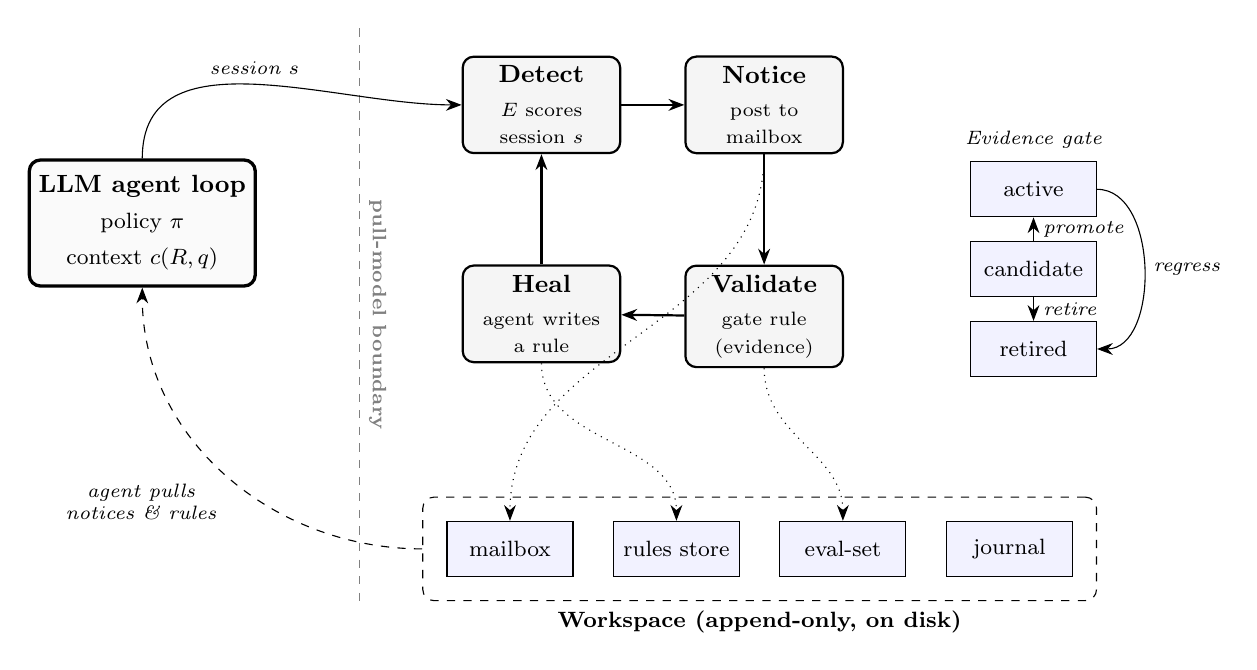
\begin{tikzpicture}[
    font=\small,
    >={Stealth[length=2mm]},
    stage/.style={draw, rounded corners, align=center, minimum width=20mm,
                  minimum height=9mm, fill=black!4, thick},
    store/.style={draw, align=center, minimum width=16mm, minimum height=7mm,
                  fill=blue!5, font=\footnotesize},
    agent/.style={draw, rounded corners, align=center, minimum width=26mm,
                  minimum height=16mm, fill=black!2, very thick},
    lbl/.style={font=\scriptsize\itshape, align=center},
    node distance=9mm and 12mm,
]

% --- Agent side (left) ---
\node[agent] (agent) {\textbf{LLM agent loop}\\[2pt]\footnotesize policy $\pi$\\[2pt]
                      \footnotesize context $c(R,q)$};

% --- Four stages of the loop (right), arranged in a cycle ---
\node[stage, right=26mm of agent, yshift=15mm] (detect)  {\textbf{Detect}\\[1pt]\scriptsize $E$ scores\\[-1pt]\scriptsize session $s$};
\node[stage, right=8mm of detect]              (notice)  {\textbf{Notice}\\[1pt]\scriptsize post to\\[-1pt]\scriptsize mailbox};
\node[stage, below=14mm of notice]             (validate){\textbf{Validate}\\[1pt]\scriptsize gate rule\\[-1pt]\scriptsize (evidence)};
\node[stage, below=14mm of detect]             (heal)    {\textbf{Heal}\\[1pt]\scriptsize agent writes\\[-1pt]\scriptsize a rule};

% cyclic arrows Detect -> Notice -> Heal -> Validate -> Detect
\draw[->, thick] (detect) -- (notice);
\draw[->, thick] (notice) -- (validate);
\draw[->, thick] (validate) -- (heal);
\draw[->, thick] (heal) -- (detect);

% --- Workspace substrate (bottom) ---
\node[store, below=20mm of heal, xshift=-4mm] (mailbox) {mailbox};
\node[store, right=5mm of mailbox]            (rules)   {rules store};
\node[store, right=5mm of rules]              (evalset) {eval-set};
\node[store, right=5mm of evalset]            (journal) {journal};
\begin{scope}[on background layer]
  \node[draw, dashed, rounded corners, fit=(mailbox)(journal),
        inner sep=3mm, label={[font=\footnotesize\bfseries]below:Workspace (append-only, on disk)}] (ws) {};
\end{scope}

% --- Evidence gate state machine (candidate -> active -> retired) ---
\node[store, right=16mm of validate, yshift=6mm]  (cand)  {candidate};
\node[store, above=3mm of cand]                   (act)   {active};
\node[store, below=3mm of cand]                   (ret)   {retired};
\draw[->] (cand) -- node[lbl,right]{promote} (act);
\draw[->] (cand) -- node[lbl,right]{retire}  (ret);
\draw[->] (act.east) to[out=0,in=0] node[lbl,right]{regress} (ret.east);
\node[lbl, above=1pt of act] {Evidence gate};

% --- Pull-model boundary (dashed vertical line between agent and harness) ---
\coordinate (btop) at ($(agent.north east)!0.5!(detect.north west) + (0,10mm)$);
\coordinate (bbot) at (btop |- ws.south);
\draw[dashed, gray] (btop) -- (bbot)
      node[midway, sloped, above, font=\scriptsize\bfseries, gray] {pull-model boundary};

% agent PULLS from workspace (arrow FROM workspace TO agent, labelled "pull") ...
\draw[->, dashed] (ws.west) to[out=180,in=270] node[lbl,below left]{agent pulls\\notices \& rules} (agent.south);
% ... and the loop's stages read/write the workspace (harness side only)
\draw[->, dotted] (notice.south) to[out=270,in=90] (mailbox.north);
\draw[->, dotted] (heal.south)   to[out=270,in=90] (rules.north);
\draw[->, dotted] (validate.south) to[out=270,in=90] (evalset.north);

% Detect reads the agent's session (the ONLY arrow crossing the boundary toward the harness)
\draw[->] (agent.north) to[out=90,in=180] node[lbl,above]{session $s$} (detect.west);

\end{tikzpicture}
}
\caption{\textbf{The Harness self-heal loop.} After each turn/task the evaluation service
$\evalfn$ scores the session (\textbf{Detect}); breaches and declining trends become diagnostic
notices posted to a filesystem workspace (\textbf{Notice}); the agent \emph{pulls} a notice, inspects
its own flagged traces, and authors a corrective rule (\textbf{Heal}); the rule enters as a
\emph{candidate} and is promoted to \emph{active} only after passing an evidence gate---a replay of
the captured failure or a forward trial---and retired if it regresses (\textbf{Validate}). The
dashed vertical line is the \emph{pull-model boundary}: the workspace is never injected into the
agent's conversation. \textit{(Placeholder schematic; see \texttt{figures/overview.tex} for the
author's redraw notes.)}}
\label{fig:overview}
\end{figure*}

\subsection{Agent, session, and evaluator}
\label{sec:setup-formal}

An agent is a policy $\pi$ that produces actions over a \emph{session} $s$ (the execution of
one task-trial). A session-level evaluation service $\evalfn$ maps a completed session to a
metric vector
\begin{equation}
  \mvec(s) = \bigl(m_1(s),\dots,m_d(s)\bigr) \in [0,1]^d,
  \label{eq:metricvec}
\end{equation}
with higher values better. In our setting $d{=}2$, with $m_1$ a session \emph{reliability}
score and $m_2$ a session \emph{consistency} score. The service is reached through a
command-line interface exposing a request/response contract (arguments in, JSON out); this
narrow seam is why the Harness core carries no runtime dependency on the service and can be
exercised against an in-process stand-in. Every call degrades gracefully to a \emph{pending}
(missing) score on failure, so the evaluation path never blocks or raises into the host agent
loop.

For metric $j$ with threshold $\tau_j$ (default $\tau_j{=}0.5$), the \emph{point-breach}
indicator is
\begin{equation}
  b_j(s) = \ind\!\left[\,m_j(s) \ne \varnothing \ \wedge\ m_j(s) < \tau_j\,\right],
  \label{eq:breach}
  % source: evaluation/metrics.py MetricScore.breached (strict <, None never a breach);
  %         config.py DEFAULT_THRESHOLD = 0.5
\end{equation}
i.e.\ strictly below threshold; a missing score is never a breach.

\paragraph{Trend breaches.} Point breaches catch acute failures but miss slow drift. We
additionally flag a \emph{declining trend} using a dual exponentially-weighted moving average
(EWMA) crossover. With per-metric EWMAs of spans $\sigma_{\mathrm{f}}{=}3$ and
$\sigma_{\mathrm{s}}{=}10$ (smoothing $\alpha=2/(\sigma+1)$), updated online as
\begin{equation}
  e^{(\cdot)}_t = \alpha\,m_j(s_t) + (1-\alpha)\,e^{(\cdot)}_{t-1},
  \label{eq:ewma}
\end{equation}
a metric is \emph{trend-declining} at session $s_t$ iff it has enough history and the fast
average has fallen below the slow average by a margin:
\begin{equation}
  \mathrm{decl}_j(s_t) = \ind\!\left[\, n_t \ge n_{\min} \ \wedge\ e^{\mathrm{f}}_t < e^{\mathrm{s}}_t - \kappa \,\right],
  \label{eq:trend}
  % source: evaluation/trends.py TrendDetector.update; history.py EWMA update
\end{equation}
with $n_{\min}{=}4$ (\texttt{trend\_min\_samples}) and $\kappa{=}0.05$
(\texttt{trend\_margin\_cross}). Two further opt-in signals (both off by default) extend this:
a \emph{relative breach} when a value falls a fixed drop below its own slow EWMA, and a
\emph{percentile breach} against a recent-window quantile. Each fired signal is emitted as a
\emph{signature} of the form \texttt{condition:metric} (e.g.\
\texttt{breach:agent\_reliability}), which downstream matching keys on.

\subsection{Context composition and rule retrieval}
\label{sec:retrieval}

The agent's behavior is steered by its policy-inducing context. We write it as a fixed base
context composed with a retrieved rule fragment:
\begin{equation}
  c(\Rset,q) = c_0 \oplus \rho(\Rset,q),
  \label{eq:context}
\end{equation}
where $\Rset$ is the current rule set, $q$ is a task query, and $\rho$ selects and renders
rules. The query is assembled from the (optional) task hint plus the signatures and metric
names of any pending notices, then tokenized (case-folded, tokens matching \texttt{[a-z0-9\_]+}
of length $\ge 2$), giving a query token set $Q$.
% source: hook/context.py compose_system_preamble builds q; workspace/rules.py _tokenize
Each rule $r$ carries tag tokens $T_r$ (from its tags) and text tokens $X_r$ (from its rule
text, rationale, and metric). Its relevance to $Q$ is
\begin{equation}
  \mathrm{score}(r,Q) = \frac{2\,\lvert Q \cap T_r\rvert + \lvert Q \cap (X_r \setminus T_r)\rvert}{\max(1,\lvert Q\rvert)} ,
  \label{eq:score}
  % source: workspace/rules.py _relevance -- tag weight 2.0, text weight 1.0,
  %         text excludes tag tokens, normalized by |Q|
\end{equation}
i.e.\ a tag-token match is weighted $2.0$, a (non-tag) text-token match $1.0$, and the score is
normalized by query size. Retrieval returns \emph{all} untagged (``global'') rules---which are
always eligible and exempt from the cutoff---together with the $\topk$ tagged rules by score:
\begin{equation}
  \rho(\Rset,q) = \mathrm{render}\!\Bigl( G(\Rset)\ \cup\ \operatorname*{top-}k_{\;r\in \Rset\setminus G}\ \mathrm{score}(r,Q) \Bigr),
  \label{eq:rho}
\end{equation}
with $k=8$ (\texttt{rules\_context\_topk}) and ties broken by score, then recency
(\texttt{created\_at}), then id. Rules beyond the cutoff remain reachable through a search tool
(\S\ref{sec:actionspace}), so retrieval bounds prompt cost without hiding knowledge.

\subsection{The self-heal operator}
\label{sec:healop}

The loop induces a map on the rule set. At step $t$, given the breaches $\Breach_t$ observed
from $\evalfn$,
\begin{equation}
  \Rset_{t+1} = \Heal(\Rset_t,\Breach_t) = \mathrm{gate}\bigl(\Rset_t,\ \mathrm{propose}(\Rset_t,\Breach_t)\bigr).
  \label{eq:heal}
\end{equation}
\emph{Propose} is executed by the agent itself: prompted by a standing protocol and a pulled
notice, it authors a candidate rule $r$ (with a rationale, an optional target metric, and tags
derived from the breach signature). \emph{Gate} is the evidence test of \S\ref{sec:validate}. A
newly authored rule enters as a \emph{candidate} when validation is enabled, and only as
\emph{active} when it is disabled; candidates are deduplicated against the live set by
normalized text and the live set is capped (\texttt{max\_active\_rules}$=50$).
% source: harness.py; workspace/rules.py RulesStore.add
Algorithm~\ref{alg:heal} states the full per-turn loop.

\begin{algorithm}[t]
\caption{Self-Heal Loop (per turn / task)}
\label{alg:heal}
\textbf{Input}: rule set $\Rset$, evaluator $\evalfn$, workspace $W$
\begin{algorithmic}[1]
\STATE compose context $c(\Rset,q)$ via Eq.~\eqref{eq:context}; run agent turn $\to$ session $s$
\STATE $\mvec(s) \gets \evalfn(s)$ \COMMENT{background, non-blocking}
\STATE compute breaches $\Breach$ via Eqs.~\eqref{eq:breach}, \eqref{eq:trend}
\IF{$\Breach \neq \varnothing$ and not deduplicated/cooled-down}
    \STATE post diagnostic notice to mailbox $\subset W$
    \IF{severity is an absolute breach and capture enabled}
        \STATE capture $s$ as a replayable eval-case
    \ENDIF
\ENDIF
\STATE \COMMENT{pull model: agent may now pull notices on its own initiative}
\IF{agent pulls a notice}
    \STATE agent inspects flagged traces; authors candidate rule $r$
    \STATE $\Rset \gets \Rset \cup \{r\}$ \COMMENT{candidate; unproven}
\ENDIF
\STATE \textsc{ValidateCandidates}($\Rset$) \COMMENT{Algorithm~\ref{alg:validate}}
\STATE \textbf{return} $\Rset$
\end{algorithmic}
\end{algorithm}

\subsection{Rule lifecycle as evidence-gating}
\label{sec:validate}

A candidate rule is admitted to the active set only if it passes a validator. We use two, tried
in order (replay first, forward trial as fallback), summarized in Algorithm~\ref{alg:validate}.

\paragraph{Forward-trial test.} Let $p_0$ be the baseline breach rate for the rule's
metric-scoped signature family, estimated over a pre-rule window as $p_0 = \text{(breached
sessions)}/\text{(sessions)}$, with the conservative convention $p_0 = 1$ when the window is
empty (the rule is assumed to have been firing).
% source: workspace/rules.py TrialState.baseline_rate (empty -> 1.0)
After admitting $r$, we observe $n$ subsequent sessions ($n=$ \texttt{trial\_min\_sessions};
package default $5$, lowered to $3$ in our study, \S\ref{sec:setup}) and form the trial breach
rate $\hat{p}$. We \textbf{promote} iff
\begin{equation}
  \hat{p} = 0 \quad\text{or}\quad \hat{p} \le p_0 - \dpromote,
  \label{eq:forward}
  % source: validation/validator.py ForwardTrialValidator (promote predicate)
\end{equation}
with $\dpromote = 0.05$ (\texttt{rule\_promote\_margin}); otherwise we \textbf{retire}. While
fewer than $n$ sessions have been observed the verdict is \emph{pending}.
Equation~\eqref{eq:forward} is a one-sided decision on a difference of breach proportions with
a fixed margin; it is deliberately \emph{conservative}---a rule must drive the breach rate to
zero or beat the baseline by at least $\dpromote$---trading statistical power for a low
false-promotion rate over the short windows available at inference time.

\paragraph{Replay test.} For captured failure cases $\{s_i\}$ (at most $3$) and protected win
cases (at most $2$), we re-run each under the candidate context $c(\Rset\cup\{r\},\cdot)$ via a
developer-supplied replay function $\textsc{Replay}:(\text{case},\ \text{context})\mapsto
\text{new session id}$, score the replayed session, and form per-metric deltas
\begin{equation}
  \Delta_j(s_i) = m'_j(s_i) - m_j(s_i),
  \label{eq:delta}
\end{equation}
where $m'$ is the replay score and $m$ the captured baseline. Let $\hat{\jmath}$ be the rule's
target metric. We deem the rule an \emph{improvement} iff some failure case improves on the
target,
\begin{equation}
  \exists\, i:\ \Delta_{\hat{\jmath}}(s_i) \ge \dpromote,
  \label{eq:improve}
  % source: validation/validator.py ReplayValidator._improved
\end{equation}
and we enforce a \emph{non-regression} constraint over \emph{all} cases (failures \emph{and}
wins) and \emph{all} shared metrics,
\begin{equation}
  \forall\, i,\ \forall\, j:\ \Delta_j(s_i) > -\dregress,
  \label{eq:noregress}
  % source: validation/validator.py ReplayValidator (retire if any delta <= -regress margin)
\end{equation}
with $\dregress = 0.05$ (\texttt{rule\_regress\_margin}). The decision order is
\emph{regression-dominates}: if Eq.~\eqref{eq:noregress} is violated we \textbf{retire}; else
if Eq.~\eqref{eq:improve} holds we \textbf{promote}; else if no failure case produced
comparable scores the verdict is \emph{pending}; otherwise we \textbf{retire} (no measured
improvement). After a bounded number of inconclusive replay rounds (three), validation falls
back to the forward trial. This is a \emph{paired improvement test with a multi-metric
non-regression constraint}: it asks not merely ``did the target metric go up?'' but ``did it go
up \emph{without} pushing any other metric, on any protected case, down by more than
$\dregress$?''

\begin{algorithm}[t]
\caption{\textsc{ValidateCandidates}: the evidence gate}
\label{alg:validate}
\begin{algorithmic}[1]
\FORALL{candidate $r \in \Rset$}
    \IF{replay available and attempts $< 3$}
        \STATE replay failure/win cases; deltas via Eq.~\eqref{eq:delta}
        \IF{$\exists\,i,j:\Delta_j(s_i)\le-\dregress$}
            \STATE \textbf{retire} $r$ \COMMENT{Eq.~\eqref{eq:noregress}}
        \ELSIF{$\exists\,i:\Delta_{\hat{\jmath}}(s_i)\ge\dpromote$}
            \STATE \textbf{promote} $r$ \COMMENT{Eq.~\eqref{eq:improve}}
        \ELSIF{no conclusive failure case}
            \STATE mark \emph{pending}; bump attempts
        \ELSE
            \STATE \textbf{retire} $r$ \COMMENT{no improvement}
        \ENDIF
    \ELSE
        \STATE observe $n$ sessions; form $p_0,\hat{p}$ \COMMENT{forward-trial fallback}
        \IF{$\hat{p}=0$ or $\hat{p}\le p_0-\dpromote$}
            \STATE \textbf{promote} $r$ \COMMENT{Eq.~\eqref{eq:forward}}
        \ELSIF{observed $\ge n$}
            \STATE \textbf{retire} $r$
        \ELSE
            \STATE \emph{pending}
        \ENDIF
    \ENDIF
\ENDFOR
\end{algorithmic}
\end{algorithm}

\paragraph{Eval-case capture.} A failure is captured for replay only when the notice's severity
is an \emph{absolute} breach (Eq.~\eqref{eq:breach}) and capture is enabled; the breaching
session is stored with its baseline scores and a replay input. Trend/relative/percentile
signals, being softer, do not by themselves create replay cases.
% source: hook/core.py _persist_notice (capture only when severity == "breach")

\subsection{Regression guard against forgetting}
\label{sec:regression}

Promotion protects against admitting a \emph{harmful} rule, but the active set as a whole can
still drift. A separate corpus-level guard replays the \emph{entire} eval-set (protected wins
first, then failures) under the current rule set and classifies each case from its deltas:
\begin{equation}
  \mathrm{cls}(s_i) =
  \begin{cases}
    \text{regressed} & \exists\, j:\ \Delta_j(s_i) \le -\dregress,\\[2pt]
    \text{improved}  & \text{else if } \exists\, j:\ \Delta_j(s_i) \ge \dpromote,\\[2pt]
    \text{unchanged} & \text{otherwise.}
  \end{cases}
  \label{eq:regcls}
  % source: validation/regression.py _classify (regressed checked FIRST)
\end{equation}
Regression is checked first, so it dominates. The run is \emph{clean} iff no case is classified
regressed. This provides a bounded guarantee---\emph{no admitted rule set regresses a
previously-passing case by more than $\dregress$ on any metric, within the replay coverage of
the eval-set}---and its limits are exactly that coverage: cases that cannot be replayed are
skipped (and reported as such), so the guard is only as strong as the captured corpus.

\subsection{The pull model and the healing action space}
\label{sec:actionspace}

Two design choices distinguish the Harness operationally. First, the \emph{pull model}:
notices, rules, and traces live in a filesystem workspace (mailbox, rules store, eval-set,
append-only journal), and \emph{nothing is injected into the agent's conversation}. The agent
reads them only by invoking tools, on its own initiative; a standing protocol in its system
context tells it how. This keeps the transcript clean, makes healing auditable, and avoids
fighting the host framework for control of the message stream. Second, healing is performed
through a self-diagnostic \emph{toolset} of $14$ operations---read/acknowledge notices, inspect
flagged traces and score history, browse the journal, add/retire/inspect rules, search and list
the rule set, assemble a cross-run reflection, and list/attach eval cases. Every operation
returns a structured result and never raises into the agent loop, so a malformed self-diagnosis
cannot crash the task.

\subsection{Hyperparameters}
\label{sec:hyper}

Table~\ref{tab:hyper} lists the tunable constants and their defaults; the study overrides are
noted in \S\ref{sec:setup}. All are lifted from the implementation's configuration.

\begin{table}[t]
\centering\small
\caption{Harness hyperparameters and default values (package defaults). Eval-case \emph{capture}
defaults off but is \emph{on} in the study's Harness arm so replay validation has cases to work
with; study overrides are noted in \S\ref{sec:setup}.}
\label{tab:hyper}
\begin{tabular}{@{}llc@{}}
\toprule
Symbol / knob & Meaning & Default \\
\midrule
$\tau_j$ & breach threshold & $0.5$ \\
$n_{\min}$ & trend min.\ samples & $4$ \\
$\kappa$ & trend crossover margin & $0.05$ \\
$\sigma_{\mathrm{f}},\sigma_{\mathrm{s}}$ & EWMA fast/slow spans & $3,10$ \\
$k$ & rules in context (\topk) & $8$ \\
$n$ & forward-trial window & $5$ \\
$\dpromote$ & promote margin & $0.05$ \\
$\dregress$ & regress margin & $0.05$ \\
--- & max active rules & $50$ \\
--- & max replay attempts & $3$ \\
--- & failure / win cases replayed & $3\,/\,2$ \\
--- & validation / retrieval / capture & on/on/off \\
\bottomrule
\end{tabular}
\end{table}

% =====================================================================================
\section{Experimental Setup}
\label{sec:setup}

We evaluate the Harness with a paired A/B protocol: the \emph{same} agent code, models,
prompts, and task sets in every arm, with the only difference being whether the Harness is
wired in. This isolates the effect of self-healing from the agent's underlying capability.

\subsection{Benchmarks}
We use three public agent benchmarks chosen because each exposes a reliability signal and
stresses a different competency:
\begin{itemize}\itemsep2pt
\item \textbf{Digital-work benchmark} \citep{placeholder-appworld}: multi-step tasks over apps
and APIs, scored by task- and scenario-goal completion plus a \emph{no-collateral-damage} check
(the agent must not corrupt unrelated state). We use its development split (57 tasks).
\item \textbf{Terminal-task benchmark} \citep{placeholder-terminalbench}: command-line tasks
executed in a sandbox, run through a standard agent-orchestration layer with a per-attempt
binary reward. We use a stratified subset ($\approx\!30$ tasks).
\item \textbf{Tool-calling dialogue benchmark} \citep{placeholder-tau2}: a customer-service
setting with an LLM-simulated user and an orchestrator; it reports $\passk$ natively. We use
one domain's task set.
\end{itemize}
Each benchmark's native pass/fail is the ground truth; the evaluation service's metrics drive
only the Harness's internal machinery.

\subsection{Arms}
\label{sec:arms}
\begin{itemize}\itemsep2pt
\item \textbf{A --- baseline:} the agent loop with no Harness (no preamble, no toolset, no
self-healing).
\item \textbf{B --- Harness:} the full loop---context preamble with retrieved rules, the
$14$-operation toolset, per-trial evaluation and candidate validation, eval-case capture on,
replay wired.
\item \textbf{B$'$ --- Harness, no-validation (ablation, flag-gated):} identical to B but rules
activate immediately (the gate of \S\ref{sec:validate} is bypassed). This isolates the
contribution of validation and is run only where budget permits.
\end{itemize}

\subsection{Learning and frozen-evaluation phases}
For each benchmark$\times$model, the Harness arm first runs a seeded \emph{learning} split
(\texttt{learning\_fraction}$=0.35$ of the task set) so it can accumulate and validate rules;
the baseline arm runs the same split for exposure symmetry (its learning-phase results are
flagged and excluded from the headline). Both arms then run the held-out \emph{frozen eval}
split, with the Harness arm carrying over the rules learned in the learning phase. Because
benchmark trials complete much faster than production sessions, the runner explicitly settles
the evaluation and drains candidate validation between task-trials so that notices land and
gates resolve \emph{during} the learning phase rather than after it.

\subsection{Models}
All model calls in every arm route through a single provider-abstraction layer, so the arms
differ only in Harness wiring. The matrix spans a frontier proprietary model plus a smaller
model from each of three commercial providers (a Gemini tier served via a managed cloud, a GPT
tier via its own API, and a Claude tier switchable between two backends); a representative
triad (one strong model per provider) is used for the headline runs. Trials are drawn from each
model's natural nondeterminism: current frontier models reject an explicit temperature control,
so trial-to-trial variance is \emph{intrinsic} and cannot be tuned away---a point we return to
in \S\ref{sec:limitations}.

\subsection{Trials, seeds, and estimators}
Each eval task is run $k=4$ times; we use $\ge 3$ study seeds, each shuffling task order to
counterbalance ordering effects on learning. For task set $T$ with per-trial pass indicators
$X_{t,i}\in\{0,1\}$,
\begin{align}
  \passone &= \frac{1}{|T|}\sum_{t\in T} X_{t,1}, \label{eq:pass1}\\
  \passk   &= \frac{1}{|T|}\sum_{t\in T} \prod_{i=1}^{k} X_{t,i}, \label{eq:passk}
  % source: benchmark-suite metrics module -- pass_at_1 (first trial); pass_hat_k (uses all()).
\end{align}
i.e.\ $\passone$ counts tasks whose \emph{first} trial passed and $\passk$ counts tasks whose
\emph{all} $k$ trials passed. Our central hypothesis is that the Harness raises $\passk$
(reliability) more than $\passone$ (peak capability)---equivalently, that it reduces
trial-to-trial variance.

\paragraph{Paired significance.} Comparisons are paired per task between the baseline ($B$) and
Harness ($H$) arms. Let $b$ be the number of tasks the baseline fails but the Harness passes
(improvements) and $c$ the reverse (regressions), with discordant count $\mathrm{disc}=b+c$.
\textbf{McNemar's test} uses an exact two-sided binomial when $\mathrm{disc}$ is small and a
continuity-corrected $\chi^2$ otherwise:
\begin{equation}
  p =
  \begin{cases}
    \min\!\bigl(1,\ 2\,F_{\mathrm{bin}}(\min(b,c);\ \mathrm{disc},\ \tfrac12)\bigr) & \mathrm{disc} < 25,\\[4pt]
    \displaystyle \Pr\Bigl[\chi^2_1 \ge \tfrac{(|b-c|-1)^2}{\mathrm{disc}}\Bigr] & \mathrm{disc} \ge 25,
  \end{cases}
  \label{eq:mcnemar}
  % source: benchmark-suite metrics module -- mcnemar (exact_threshold=25, Edwards correction)
\end{equation}
and a discordant count below the exact threshold ($25$) is flagged \emph{underpowered}. For the
effect size we report the paired delta $\Delta = \mathrm{rate}_H - \mathrm{rate}_B$ with a
\textbf{percentile bootstrap} $95\%$ confidence interval on the mean of the per-task
differences ($10{,}000$ resamples, fixed seed):
\begin{equation}
  \mathrm{CI}_{95} = \Bigl[\,Q_{2.5}\bigl(\{\bar{d}^{(b)}\}\bigr),\ Q_{97.5}\bigl(\{\bar{d}^{(b)}\}\bigr)\,\Bigr],
  \label{eq:bootstrap}
  % source: benchmark-suite metrics module -- bootstrap_ci, paired_delta
\end{equation}
where $\bar{d}^{(b)}$ is the mean paired difference on bootstrap resample $b$.

\subsection{Two methodological checkpoints}
\label{sec:checkpoints}
The Harness can only help if a long causal chain fires: task failure $\to$ metric breach $\to$
notice $\to$ authored rule $\to$ promotion $\to$ generalization. Two links are unverified going
in, so we gate expensive runs on them.
\begin{itemize}\itemsep2pt
\item \textbf{Checkpoint 1 (metric--failure calibration).} The evaluation metrics were designed
for production sessions; whether they correlate with \emph{benchmark} task failure is an
empirical question. After the first learning run of each benchmark we calibrate the breach
predicate against the benchmark's own pass/fail labels---precision, recall, and F1 over a
threshold sweep---and, if needed, adjust $\tau$ per the sweep (the same $\tau$ for all arms and
seeds of a benchmark). \emph{If no threshold yields usable signal, arm B is inert and we report
that null mechanism as a finding rather than papering over it.}
\item \textbf{Checkpoint 2 (rules promoted before eval).} With a short learning phase, the
Harness may reach frozen eval with zero \emph{active} rules, making arm B ``baseline plus
overhead.'' We therefore lower the forward-trial window to $n=3$ for the study and inspect the
archived workspace after learning; if zero rules were promoted we flag the run accordingly so
analysis can separate ``learned nothing'' from ``rules didn't help.''
\end{itemize}

\subsection{The token-overhead confound}
\label{sec:confound}
The Harness arm pays a context cost on every turn: the rule preamble plus $14$ extra tool
definitions consume input tokens whether or not any rule fires, which can depress performance
on long tasks independently of rule quality. We treat this as a confound to \emph{report, not
fix}: the cost/overhead table (\S\ref{sec:telemetry}) quantifies the added tokens and latency
per turn so that any effect on $\passk$ can be read alongside its price.

\begin{table}[t]
\centering\small
\caption{Configuration matrix (placeholder; per-benchmark counts finalized by seed).}
\label{tab:config}
\begin{tabular}{@{}lccccc@{}}
\toprule
Benchmark & Split & \#learn & \#eval & $k$ & turns \\
\midrule
Digital  & dev      & \TBD & \TBD & 4 & 100 \\
Terminal & subset   & \TBD & \TBD & 4 & 100 \\
Dialogue & 1 domain & \TBD & \TBD & 4 & 100 \\
\midrule
\multicolumn{6}{@{}l}{\small Seeds $\{1,2,3\}$; arms A, B, B$'$; forward-trial window $n{=}3$.} \\
\bottomrule
\end{tabular}
\end{table}

% =====================================================================================
\section{Results and Discussion}
\label{sec:results}

\noindent\textbf{Note.} The study's benchmark runs are in progress. Every numeric cell in this
section is a placeholder (\TBD); the tables define the exact columns and the analysis reads them
once the runs land. We present the interpretation scaffolding so the empirical claims can be
evaluated the moment numbers are filled in.

\subsection{Main results}
\label{sec:main}
Table~\ref{tab:headline} is the headline comparison: for each benchmark$\times$model,
$\passone$ and $\passk$ under baseline and Harness, the paired deltas, a bootstrap $95\%$ CI on
the delta, and the McNemar $p$-value (Eqs.~\eqref{eq:pass1}--\eqref{eq:bootstrap}). The
hypothesis predicts a \emph{larger} positive $\Delta\passk$ than $\Delta\passone$: if the
Harness mainly removes trial-to-trial failures, the ``all-$k$-pass'' rate should rise more than
the ``first-trial-pass'' rate. A positive $\Delta\passk$ whose CI excludes zero, with a small
McNemar $p$, would support the claim; a positive $\Delta\passone$ with a flat $\Delta\passk$
would instead indicate a capability bump without a reliability gain. Because subsets are
modest, we read effects as \emph{directional with CIs} and do not over-interpret small deltas
(\S\ref{sec:limitations}).

\begin{table*}[t]
\centering\small
\caption{Headline results (placeholder). Baseline (B) vs.\ Harness (H); $\Delta = \mathrm{H}-\mathrm{B}$.
CI is a percentile bootstrap $95\%$ interval on the paired $\passk$ delta; $p$ is McNemar's test on
paired outcomes. \emph{Numbers forthcoming pending completion of the runs.}}
\label{tab:headline}
\begin{tabular}{@{}llcccccccc@{}}
\toprule
& & \multicolumn{3}{c}{$\passone$} & \multicolumn{3}{c}{$\passk$} & & \\
\cmidrule(lr){3-5}\cmidrule(lr){6-8}
Benchmark & Model & B & H & $\Delta$ & B & H & $\Delta$ & CI$_{95}(\Delta\passk)$ & McNemar $p$ \\
\midrule
Digital-work  & frontier & \TBD & \TBD & \TBD & \TBD & \TBD & \TBD & \TBD & \TBD \\
Digital-work  & small    & \TBD & \TBD & \TBD & \TBD & \TBD & \TBD & \TBD & \TBD \\
Terminal-task & frontier & \TBD & \TBD & \TBD & \TBD & \TBD & \TBD & \TBD & \TBD \\
Terminal-task & small    & \TBD & \TBD & \TBD & \TBD & \TBD & \TBD & \TBD & \TBD \\
Tool-dialogue & frontier & \TBD & \TBD & \TBD & \TBD & \TBD & \TBD & \TBD & \TBD \\
Tool-dialogue & small    & \TBD & \TBD & \TBD & \TBD & \TBD & \TBD & \TBD & \TBD \\
\bottomrule
\end{tabular}
\end{table*}

\subsection{Learning dynamics}
\label{sec:learning}
Figure~\ref{fig:results} plots the Harness arm's pass rate over the learning phase alongside
the cumulative count of \emph{promoted} rules. The mechanism predicts an upward pass-rate trend
that tracks rule promotions and then plateaus as the rule set saturates; a flat pass rate
despite promotions would suggest the promoted rules do not generalize within the learning
split. This figure is also where Checkpoint~2 (\S\ref{sec:checkpoints}) is read: if the
promoted-rules curve never leaves zero, arm B was effectively baseline-plus-overhead for that
run.

\begin{figure}[t]
\centering
\resizebox{\columnwidth}{!}{% figures/results.tex  --  Figure 2: results placeholder (arm-B learning dynamics).
%
% AUTHOR TODO: Replace with the real plot once the learning-phase runs land. Two options
% (pick one for camera-ready; this placeholder sketches the learning-curve variant):
%
%   OPTION A (shown here) -- Learning dynamics, arm B only:
%       x-axis = learning task-trial index (each trial is one session);
%       left y-axis = cumulative/rolling pass rate (0..1) of the harness arm;
%       right y-axis = cumulative count of PROMOTED (active) rules.
%     Expected/hypothesised shape: pass rate trends UP and to the right as rules are
%     promoted; the promoted-rules step function rises then plateaus (rule set saturates).
%     A flat pass-rate line would indicate the harness learned nothing useful (null result).
%
%   OPTION B -- pass@1-vs-pass^k deltas: grouped bars per (benchmark x model), showing
%     Delta pass@1 and Delta pass^k (harness - baseline). Hypothesis: Delta pass^k > Delta pass@1
%     (reliability rises more than peak capability).
%
% Drawn with base TikZ only (no pgfplots dependency); main.tex wraps this in \resizebox so it
% always fits the column regardless of internal size. The curve below is ILLUSTRATIVE /
% SCHEMATIC -- it encodes the *expected shape*, NOT measured data; axes carry no numeric ticks.

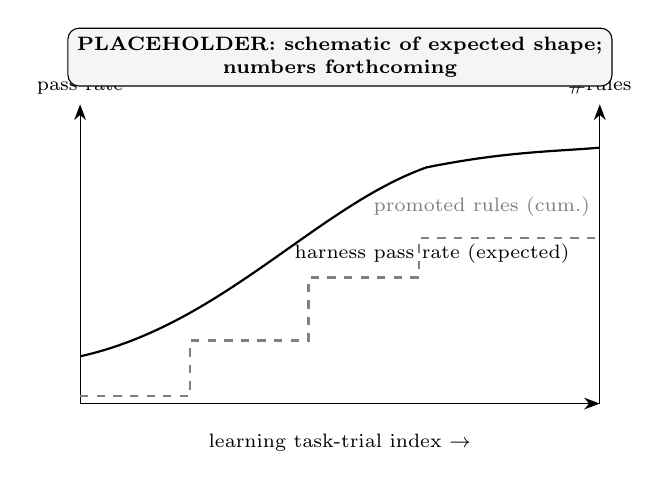
\begin{tikzpicture}[font=\small, >={Stealth[length=2mm]}]
  \def\W{66mm} \def\H{38mm}
  % axes
  \draw[->] (0,0) -- (\W,0);
  \draw[->] (0,0) -- (0,\H) node[above, font=\scriptsize] {pass rate};
  \draw[->] (\W,0) -- (\W,\H) node[above, font=\scriptsize] {\#rules};
  \node[font=\scriptsize] at (0.5*\W,-5mm) {learning task-trial index $\rightarrow$};

  % SCHEMATIC pass-rate curve (rising, concave) -- illustrative only, not data
  \draw[thick, black]
      (0,6mm) .. controls (18mm,10mm) and (30mm,25mm) .. (44mm,30mm)
              .. controls (54mm,32mm) and (60mm,32mm) .. (\W,32.5mm);
  \node[font=\scriptsize, black, anchor=west] at (26mm,19mm) {harness pass rate (expected)};

  % SCHEMATIC cumulative promoted-rules step function -- illustrative only
  \draw[thick, dashed, gray]
      (0,1mm) -- (14mm,1mm) -- (14mm,8mm) -- (29mm,8mm) -- (29mm,16mm)
      -- (43mm,16mm) -- (43mm,21mm) -- (\W,21mm);
  \node[font=\scriptsize, gray, anchor=east] at (\W,25mm) {promoted rules (cum.)};

  % TBD banner
  \node[draw, fill=black!4, rounded corners, font=\scriptsize\bfseries, align=center]
       at (0.5*\W, \H+6mm) {PLACEHOLDER: schematic of expected shape;\\numbers forthcoming};
\end{tikzpicture}
}
\caption{\textbf{Learning dynamics (placeholder, schematic).} Harness-arm pass rate (solid) and
cumulative promoted rules (dashed) vs.\ learning task-trial index. The curves show the
\emph{expected shape}, not measured data; axes carry no numeric ticks. See
\texttt{figures/results.tex} for the author's redraw notes and the alternative
$\Delta\passone$-vs-$\Delta\passk$ bar variant.}
\label{fig:results}
\end{figure}

\subsection{Harness telemetry and cost}
\label{sec:telemetry}
Table~\ref{tab:telemetry} reports what the Harness actually did---rules proposed, promoted, and
retired; notices raised; the breach rate; and the mean number of rules rendered into
context---next to its price: added input tokens per turn and latency overhead versus baseline.
This table lets a reader weigh any reliability gain against the token-overhead confound
(\S\ref{sec:confound}): a gain in $\passk$ accompanied by a large per-turn token premium is a
different result than the same gain at near-zero overhead. It also surfaces degenerate
regimes---many notices but no promotions (the gate rejecting everything), or promotions with no
measured gain (rules that pass the gate but do not generalize).

\begin{table}[t]
\centering\small
\caption{Harness telemetry and overhead (placeholder). Grouped per run/phase.
\emph{Numbers forthcoming.}}
\label{tab:telemetry}
\begin{tabular}{@{}lccc@{}}
\toprule
Quantity & Digital & Terminal & Dialogue \\
\midrule
rules proposed        & \TBD & \TBD & \TBD \\
rules promoted        & \TBD & \TBD & \TBD \\
rules retired         & \TBD & \TBD & \TBD \\
notices raised        & \TBD & \TBD & \TBD \\
breach rate           & \TBD & \TBD & \TBD \\
mean rules in context & \TBD & \TBD & \TBD \\
added tokens / turn   & \TBD & \TBD & \TBD \\
latency overhead      & \TBD & \TBD & \TBD \\
\bottomrule
\end{tabular}
\end{table}

\subsection{Ablations}
\label{sec:ablations}
Table~\ref{tab:ablation} isolates the contribution of each design choice against the full
Harness:
\begin{itemize}\itemsep2pt
\item \textbf{No-validation} (arm B$'$): rules activate immediately. This isolates the
\emph{evidence gate}. If validation matters, removing it should \emph{lower} $\passk$ (unproven
rules, including harmful ones, take effect)---and it may raise variance.
\item \textbf{No-retrieval:} all active rules are rendered rather than the $\topk$ relevant
ones (Eq.~\eqref{eq:rho}). This isolates \emph{task-conditioned retrieval}; the expected effect
is higher token cost and, on larger rule sets, distraction that can erode $\passk$.
\item \textbf{Replay-only} and \textbf{forward-trial-only:} restrict the gate to a single
validator. Replay-only cannot promote rules for which no replayable case was captured;
forward-trial-only is slower to promote and cannot use counterfactual replay evidence. These
isolate the two halves of \S\ref{sec:validate}.
\end{itemize}
Each row is reported as $\Delta$ versus the full Harness, so the sign and magnitude directly
read out the value of the removed component.

\begin{table}[t]
\centering\small
\caption{Ablations (placeholder), aggregated over benchmarks/models. $\Delta$ is relative to the
full Harness. \emph{Numbers forthcoming.}}
\label{tab:ablation}
\begin{tabular}{@{}lccc@{}}
\toprule
Variant & $\passone$ & $\passk$ & $\Delta\passk$ vs.\ full \\
\midrule
Full Harness         & \TBD & \TBD & --- \\
\ \ no-validation (B$'$) & \TBD & \TBD & \TBD \\
\ \ no-retrieval     & \TBD & \TBD & \TBD \\
\ \ replay-only      & \TBD & \TBD & \TBD \\
\ \ forward-trial-only & \TBD & \TBD & \TBD \\
\bottomrule
\end{tabular}
\end{table}

\subsection{Limitations and threats to validity}
\label{sec:limitations}
We flag the following, honestly, ahead of the completed runs.

\paragraph{Statistical power.} At $\approx\!30$--$40$ eval tasks per benchmark, McNemar detects
only large deltas (Eq.~\eqref{eq:mcnemar} flags $\mathrm{disc}<25$ as underpowered); even
pooling seeds, small effects will not be significant. We therefore present results as
directional with CIs and scale subsets up only where early deltas look promising.

\paragraph{Dependence on the breach signal.} The whole mechanism is downstream of the
evaluation service's metrics tracking task failure. Checkpoint~1 (\S\ref{sec:checkpoints})
tests this correlation directly; if it is weak, arm B is inert regardless of rule quality, and
that is itself a reportable outcome.

\paragraph{Token-overhead confound.} As in \S\ref{sec:confound}, the preamble and toolset cost
tokens every turn; a $\passk$ change must be read next to Table~\ref{tab:telemetry}.

\paragraph{Benchmark-integration coverage.} Our integrations differ in how thoroughly they were
exercised at build time. The digital-work integration was verified end-to-end against a live
environment server (with a scripted tool call; a full live-model end-to-end run was not
executed). The terminal-task and tool-dialogue integrations were implemented against the
benchmarks' real APIs but were \emph{not} run end-to-end at build time (they were exercised
only through the mock/dry-run pipeline). The statistical machinery
(Eqs.~\eqref{eq:pass1}--\eqref{eq:bootstrap}) is unit-tested but has not yet been run on real
study data, and both checkpoints of \S\ref{sec:checkpoints} are built but unexecuted---so no
calibration F1 or rule-promotion counts exist yet. We will update these as runs complete.

\paragraph{Intrinsic trial variance.} Because the models reject temperature control, we cannot
suppress sampling variation; the learning phase is therefore mildly nondeterministic across
seeds, which we counterbalance by seed and task-order shuffling but cannot eliminate.

\paragraph{Generality.} Results are specific to the tested domains, the two session-quality
metrics, and text-only rules; whether the loop transfers to other metrics, richer rule
representations, or other agent architectures is open (\S\ref{sec:conclusion}).

% =====================================================================================
\section{Conclusion and Future Work}
\label{sec:conclusion}

We presented a self-healing agent harness that closes the loop on agent \emph{reliability}: it
detects its own degradations, lets the agent author corrective rules, and---unlike open-loop
self-correction---admits each rule only after it passes an empirical evidence gate, with a
regression guard against forgetting. We cast the loop as an evidence-gated operator on the
agent's policy-inducing context and gave the exact retrieval, promotion, and regression
predicates used in our implementation, together with a three-benchmark A/B protocol for
measuring the $\passone$ vs.\ $\passk$ reliability gap. The empirical verdict is forthcoming.

Several directions follow. \textbf{Richer rule representations}---structured or parameterized
rules, or rules with preconditions---could raise the ceiling on what a single promotion can
fix. \textbf{Multi-metric, vector-valued validation} would replace the scalar
target/non-regression split of \S\ref{sec:validate} with a Pareto criterion.
\textbf{Cross-agent rule sharing} raises the question of when a rule validated for one agent
transfers to another. On the theory side, the self-heal operator $\Heal$ (Eq.~\eqref{eq:heal})
invites a \textbf{regret/convergence analysis}: under what conditions does gated adaptation
converge, and how does the promote margin trade false promotions against learning speed?
Finally, \textbf{online threshold adaptation} would let $\tau$ track a benchmark or deployment
automatically, and \textbf{human-in-the-loop} variants could interpose review before promotion
where stakes warrant it.

% =====================================================================================
% The aaai2027 style sets the bibliographystyle (aaai2027.bst) automatically -- do not add
% a \bibliographystyle command here.
\bibliography{references}

\end{document}
